\vspace*{3pc}
\begin{center}
\begin{minipage}{0.7\linewidth}
\hrule
\vspace{8pt}
{\huge\guillemotleft} ~One should never try to prove anything that is not almost obvious. {\huge\guillemotright}  \\
\vspace{2pt}
\begin{flushright}
--- \textsc{Alexander Grothendieck}
\end{flushright}
\vspace{8pt}
\hrule
\end{minipage}
\end{center}
\vspace{3pc}


%\section*{Introduction}

\begin{intro}
{\color{purple}I}mplementing non-cold dark matter particles in our simulations was no trivial task, and constituted a significant fraction of my PhD. Nonetheless, the Ly-$\alpha$ group in Saclay is now fully implicated on the international stage when it comes to investigating hot, warm, cool and cold dark matter cosmologies. When I was introduced to the Ly-$\alpha$ group in Saclay early in my PhD, it was already well involved in the investigation of constraining sub-$eV$ neutrino masses in the context of a cold+hot dark matter cosmology (\textit{a.k.a.} $\Lambda$CDM$\nu$). Our working group had already published the tightest constraints to date on $\sum m_\nu$ (see \cite{Palanque2015a}). I contributed to further improving those constraints by modeling several systematic uncertainty levels which I've described in Chap.~\ref{chap:Simulations}. I detail the most up-to-date constraints on $\sum m_\nu$ obtained in the final section of this chapter. Once familiar with our methodology described in Sec.~\ref{sec:methodology}, I chose to investigate three projects in addition to the aforementioned C+HDM: sterile neutrino dark matter as a candidate particle for a (1) purely WDM, (2) mixed C+WDM and (3) purely cool DM. These topics of research were new to the Saclay group and I carried most of the work from the preliminary bibliographical status to contacts with experts in the field, and finally their implemention into the simulation pipeline to produce the results stated in this manuscript. In this chapter, I lay out the results on all four of these projects. In each one, I quote constraints from the Ly-$\alpha$ forest power spectrum using our BOSS DR9 sample as well as in combination with higher resolution data sets, \textit{i.e.} XQ-100, MIKE and HIRES. In all four projects, the bounds on non-CDM particle mass we obtain are amongst the most competitive to date. Finally, in each project, I lay the main caveats and bottleneck issues that require further investigation.
\end{intro}

\begin{figure}
\begin{center}
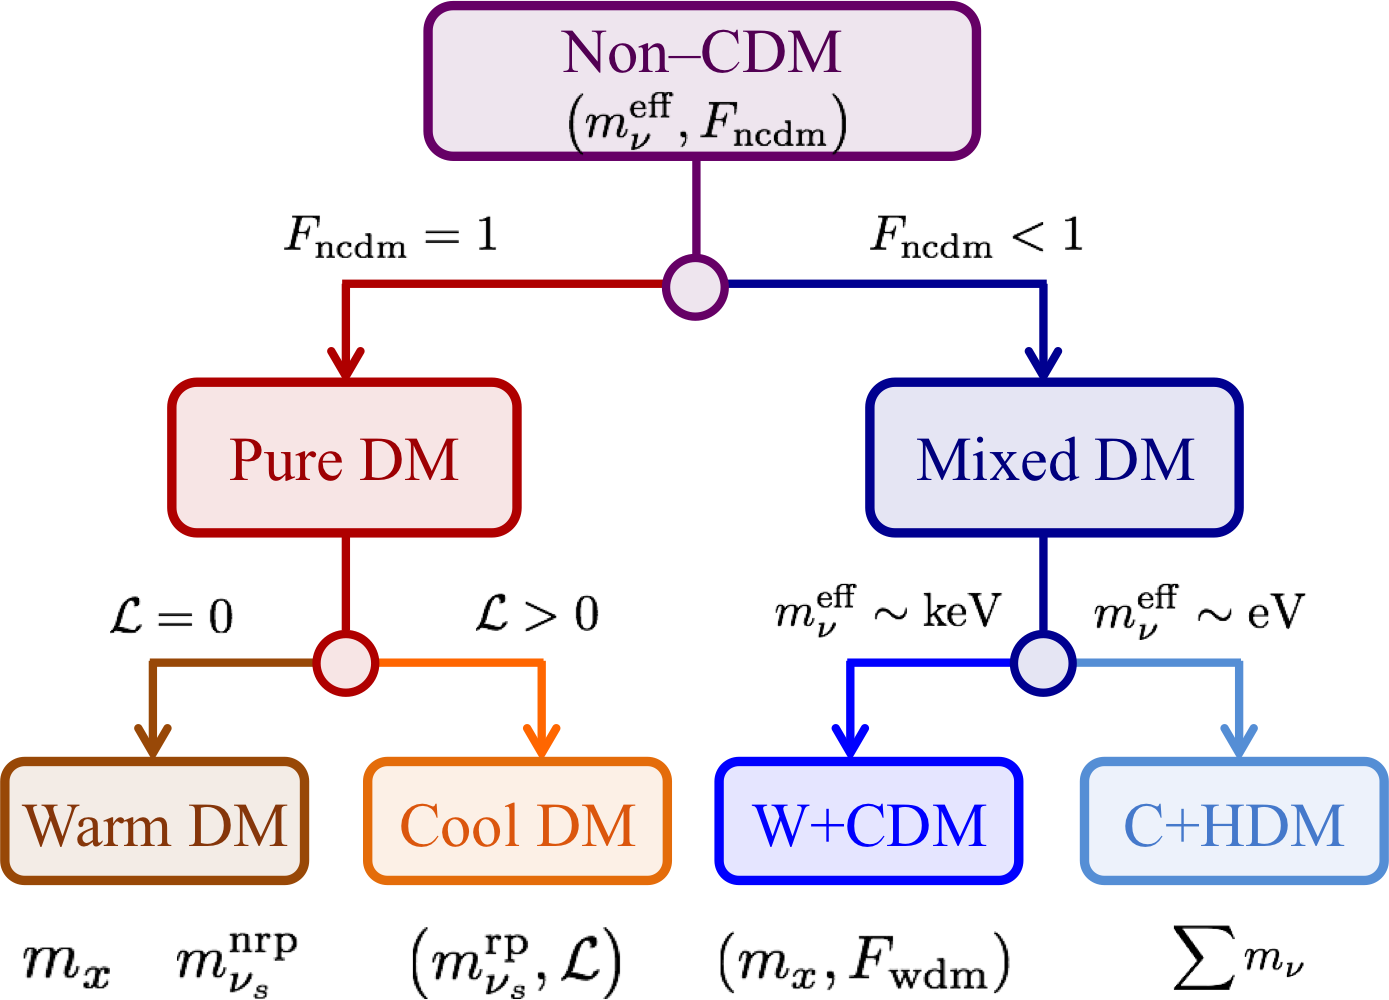
\includegraphics[width=0.8\columnwidth]{Project_Outline.png}
\caption{Schematic workflow of the 4 non-cold dark matter projects I investigate, along with the relevant parameters involved. The non-cold to cold dark matter ratio differentiates between pure dark matter ($F_{\mathrm{ncdm}} = 1$) and mixed dark matter ($F_{\mathrm{ncdm}} < 1$) cosmologies. In the former, the warm and cool dark matter projects are distinguished by the value of the net leptonic asymmetry parameter. In the latter, the cold plus warm and cold plus hot dark matter projects are distinguished by the rest mass scale of the effective neutrino mass.}
\label{fig:outline}
\end{center}
\end{figure}
